\def\QRCODE{MASTER_mispa_TUT.IMG.morphological_geodesic_filtering_pythonqrcode.png}
\def\QRPAGE{http://www.iptutorials.science/tree/master/MASTER_mispa/TUT.IMG.morphological_geodesic_filtering/python}
\mcorrectionsection{Python correction}

\begin{python}
from skimage.util import random_noise
from scipy import misc
import matplotlib.pyplot as plt
from skimage import morphology as m
from skimage import filters
import numpy as np
\end{python}

\subsection{Morphological center}
The noisy image is obtained with the function \pinline{random_noise} from \pinline{skimage.util}.

\begin{python}
L = imageio.imread('lena512.bmp');
A = random_noise(L, mode='s&p', amount=.04);
\end{python}

Following the definition, the morphological center is obtained with the following code, and illustrated in Fig.\ref{fig:geodesic_filtering:python:center}:
\begin{python}
def morphoCenter(I, c, o, selem=m.disk(1)):
    """
    """
    coc = c(o(c(I, selem=selem), selem=selem), selem=selem);
    oco = o(c(o(I, selem=selem), selem=selem), selem=selem);
    cMin = np.minimum(oco, coc);
    cMax = np.maximum(oco, coc);
    F = np.minimum( np.maximum(A, cMin), cMax);
    return F;

B = morphoCenter(A, m.closing, m.opening);
Bmed= filters.median(A, selem=np.ones((3,3)));
\end{python}

\begin{figure}[H]
 \centering\caption{Morphological center compared to the classical median filter.}
%  \subfloat[Original image.]{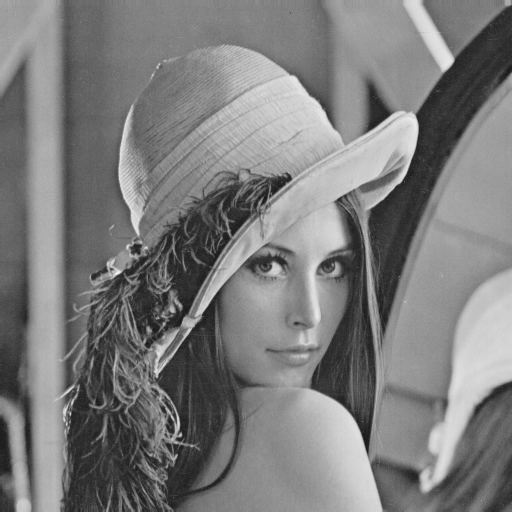
\includegraphics[width=.3\linewidth]{lena512.png}}
%  \hspace{1cm}
 \subfloat[Noisy image.]{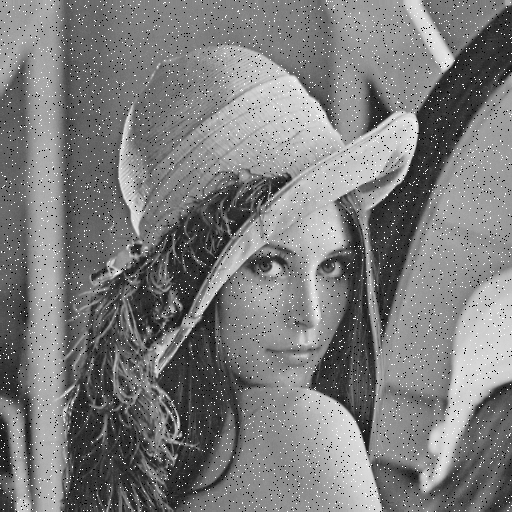
\includegraphics[width=.3\linewidth]{noisy_lena.python.png}}
 \hfill
 \subfloat[Median filter of size $5\times 5$.]{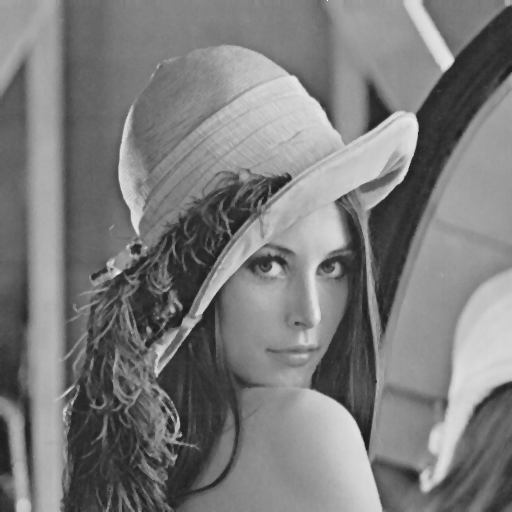
\includegraphics[width=.3\linewidth]{median.python.png}}
 \hfill
 \subfloat[Morphological center.]{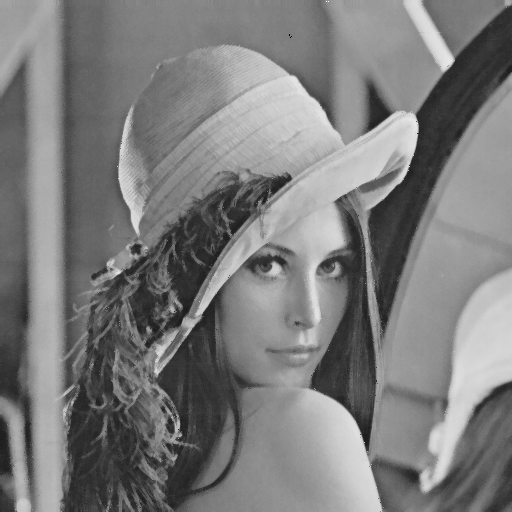
\includegraphics[width=.3\linewidth]{morpho_center.python.png}}%
 \label{fig:geodesic_filtering:python:center}%
\end{figure}


\subsection{Alternate sequential filters}
The order of these filters are often chosen empirically. The results are illustrated in Fig.\ref{fig:geodesic_filtering:python:asf}.

\begin{python}
def asf_n(I, order=3):
    F = I.copy();
    for r in np.arange(1, order+1):
        se = m.disk(r);
        F = m.opening( m.closing(F, selem=se), selem=se);
    return F;
\end{python}

\begin{python}
def asf_m(I, order=3):
    F = I.copy();
    for r in np.arange(1, order+1):
        se = m.disk(r);
        F = m.closing( m.opening(F, selem=se), selem=se);
    return F;
\end{python}

\begin{figure}[H]
 \centering\caption{Alternate Sequential Filters compared to original image.}%
 \subfloat[Original image.]{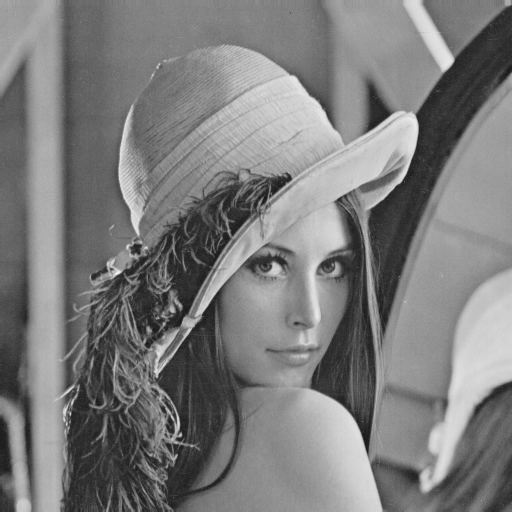
\includegraphics[width=.3\linewidth]{lena512.png}}
 \hfill
 \subfloat[ASF of order 3, starting with a closing operation (denoted N).]{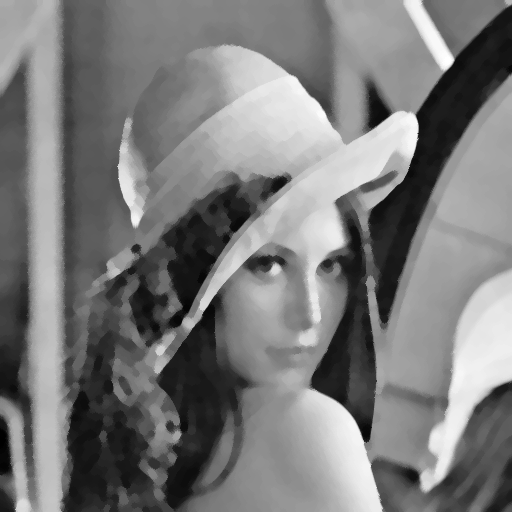
\includegraphics[width=.3\linewidth]{asf_n.python.png}}
 \hfill
 \subfloat[ASF of order 3, starting with an opening operation (denoted M).]{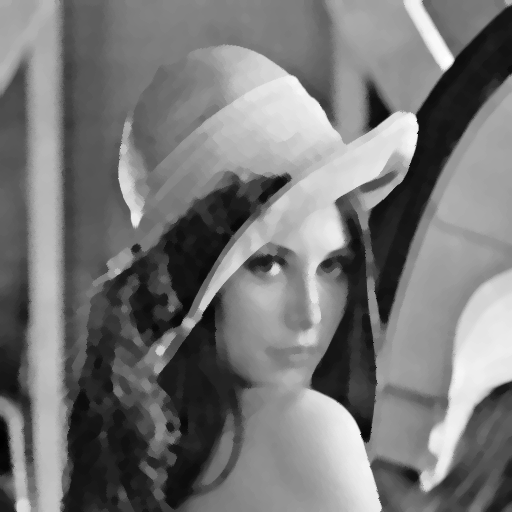
\includegraphics[width=.3\linewidth]{asf_m.python.png}}%
 \label{fig:geodesic_filtering:python:asf}%
\end{figure}

\subsection{Geodesic reconstruction filters}
These two functions are simply implemented using erosion and reconstruction operators. Notice the duality property, that is used to code \pinline{closerec}. In this example, 8 bits images (unsigned) are considered, and the results are illustrated in Fig.\ref{fig:geodesic_filtering:python:georec}.

\begin{python}
def openrec(I, selem=m.disk(1)):
    B = m.erosion(I, selem=selem);
    F = m.reconstruction(B, I);
    return F;
\end{python}

\begin{python}
def closerec(I, selem=m.disk(1)):
    F = 255-openrec(255-I, selem=selem);
    return F;
\end{python}

\begin{figure}[H]
 \centering\caption{Opening and closing by reconstruction.}%
 \subfloat[Original image.]{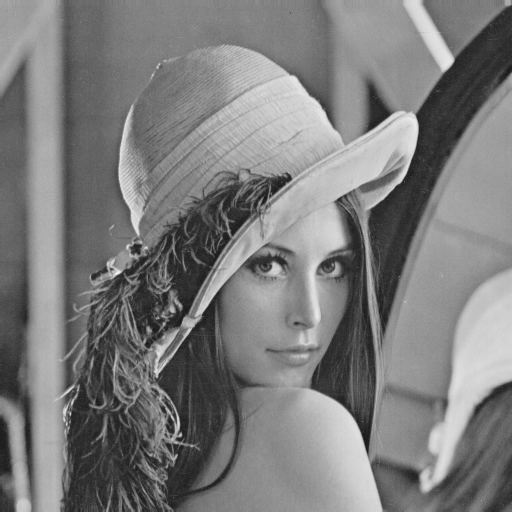
\includegraphics[width=.3\linewidth]{lena512.png}}
 \hfill
 \subfloat[Opening by reconstruction.]{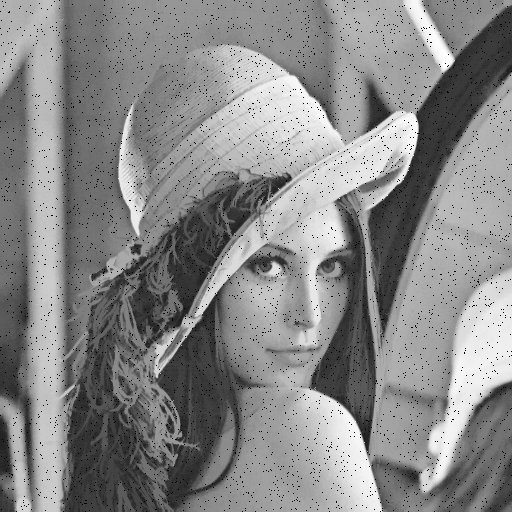
\includegraphics[width=.3\linewidth]{lena_openrec.python.png}}
 \hfill
 \subfloat[Closing by reconstruction.]{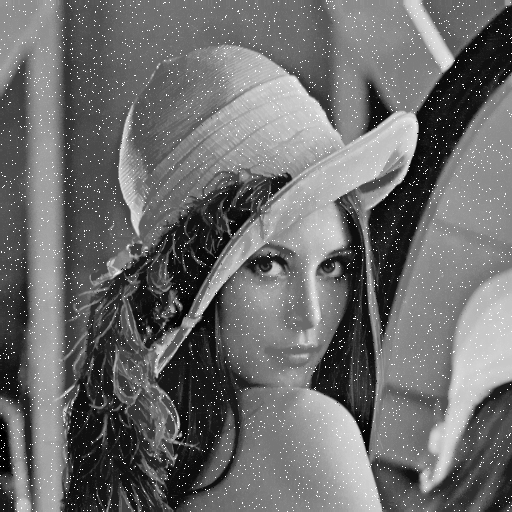
\includegraphics[width=.3\linewidth]{lena_closerec.python.png}}%
 \label{fig:geodesic_filtering:python:georec}%
\end{figure}

\subsection{ASF by reconstruction}
This is an example of a 3rd order alternate sequential filter, illustrated in Fig.\ref{fig:geodesic_filtering:python:asf_rec}.

\begin{python}
def asfrec(I, order=3):
    A = I.copy();
    for r in np.arange(1, order+1):
        se = m.disk(r);
        A = closerec(openrec(A, selem=se), selem=se);
    return A;
\end{python}

\begin{figure}[htbp]
 \centering\caption{Alternate Sequential Filtering by reconstruction.}%
 \subfloat[Original image.]{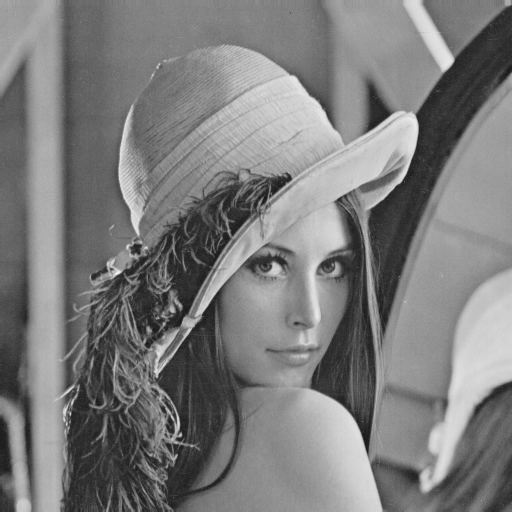
\includegraphics[width=.3\linewidth]{lena512.png}}
 \hfill
 \subfloat[ASF of order 3 by reconstruction.]{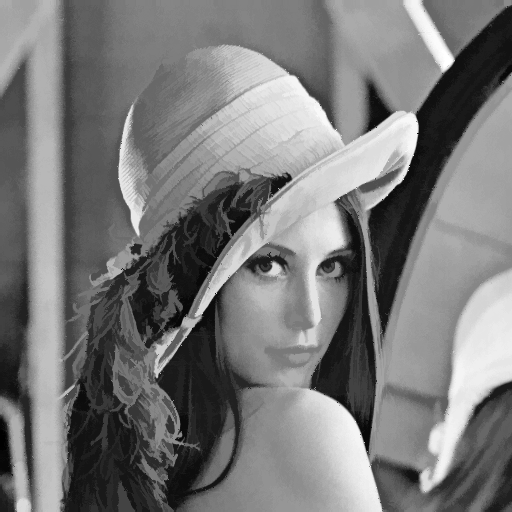
\includegraphics[width=.3\linewidth]{asfrec.python.png}}
 \hfill
 \subfloat[Noisy image.]{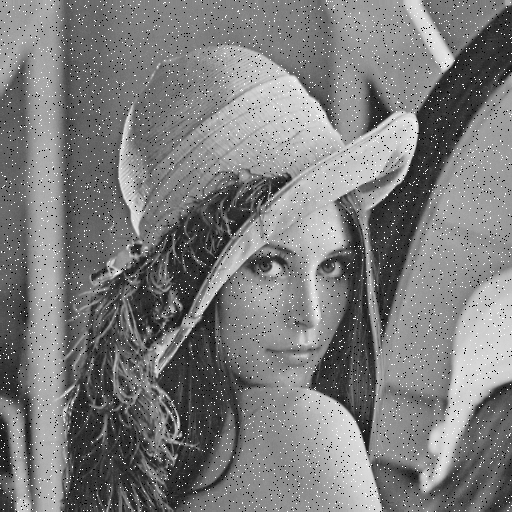
\includegraphics[width=.3\linewidth]{noisy_lena.python.png}}%
 \label{fig:geodesic_filtering:python:asf_rec}%
\end{figure}

\subsection{Morphological center by reconstruction}
Morphological center by reconstruction replaces the opening and closing operations by their equivalent by reconstruction (see Fig.\ref{fig:geodesic_filtering:python:center_rec}).

\begin{python}
def centerrec(I, selem=m.disk(1)):
    """
    """
    B = morphoCenter(I, closerec, openrec, selem=selem);
    return B;
\end{python}

\begin{figure}[htbp]
 \centering\caption{Morphological center by reconstruction.}
 \subfloat[Original image.]{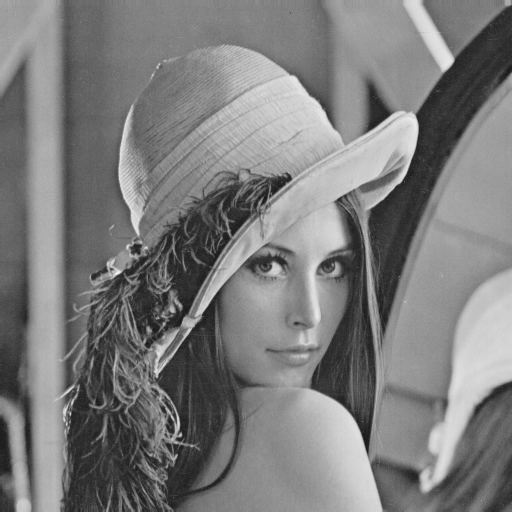
\includegraphics[width=.3\linewidth]{lena512.png}}
 \hfill
 \subfloat[Center by reconstruction.]{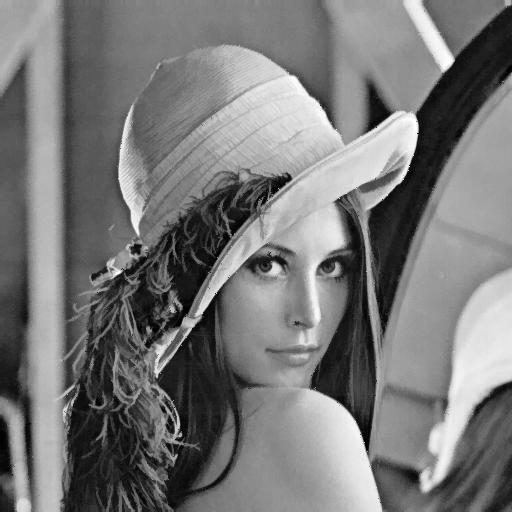
\includegraphics[width=.3\linewidth]{centerrec.python.png}}
 \hfill
 \subfloat[Noisy image.]{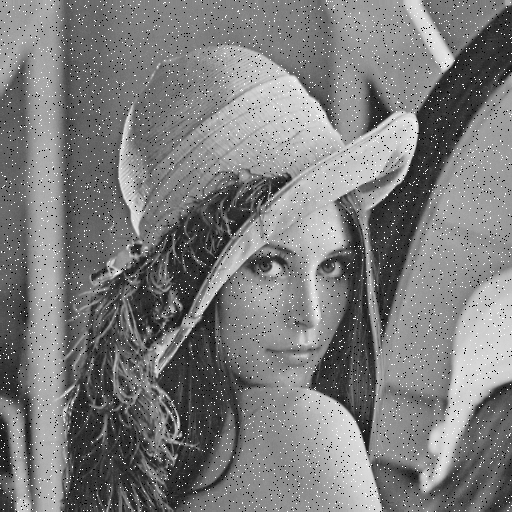
\includegraphics[width=.3\linewidth]{noisy_lena.python.png}}%
 \label{fig:geodesic_filtering:python:center_rec}%
\end{figure}